\documentclass[]{article}
\usepackage[margin={1in}]{geometry}
\usepackage[english]{babel}
\usepackage{datetime}
\usepackage{amsmath}
\usepackage{listings}
\usepackage{verbatim}
\usepackage{fancyhdr}
\usepackage[obeyspaces]{url}
\usepackage{graphicx}
\usepackage{tikz}
\usetikzlibrary{automata, positioning, arrows}
\graphicspath{ {.} }
\newcommand{\class}{TC2006. Programming Languages}
\newcommand{\hwname}{Homework 03}
\pagestyle{fancy}
\fancyhf{}
\lhead{\class \\ \hwname}
\rhead{Andrés Alam Sánchez Torres (A00824854) \\ \today}
\lstset{breaklines=true} 

\begin{document}
    \setlength{\headheight}{23.10004pt}
    \addtolength{\topmargin}{-11.10004pt}    

    \noindent
    In this homework, you will use the strategies seen in class to design a scanner that detects 
    valid words of simple toy languages. This homework may be solved in teams of at most three 
    members. If you want, you can submit this homework individually.

    To simplify this homework, assume that you can use DIGITS or LETTERS to refer to the digits 
    (characters 0 to 9) or the upper case letters in the English alphabet (characters A to Z), 
    respectively. If you need it, you can even use natural language to express a particular condition.

    \section{Designing a DFA - Case I}
    Design a DFA that recognizes the lexical elements defined by the following information.

    \begin{itemize}
        \item[] \textbf{NUMBER.} At least one digit followed by zero or more digits. \textbf{Recognized by $q_{101}$/}
        \item[] \textbf{VARIABLE.} The symbol \$ followed by any combination of letters and digits, as long as they start with a letter. \textbf{Recognized by $q_{102}$/}
        \item[] \textbf{OPERATOR.} Any of the following characters: +, -, *, or /. \textbf{Recognized by $q_{103}$/}
    \end{itemize}

    \begin{center}
        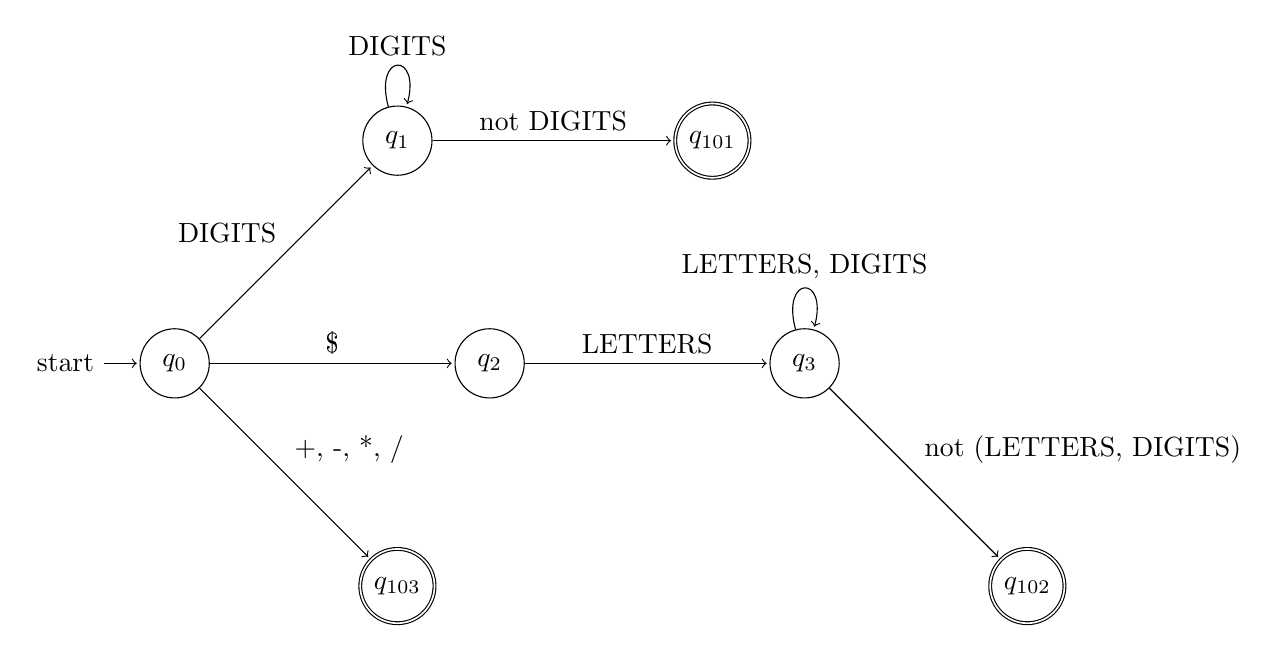
\begin{tikzpicture}[shorten >=1pt,node distance=4cm,on grid,auto] 
            \node[state, initial] (q_0) {$q_0$};
            \node[state] (q_1) [above right=of q_0] {$q_1$}; 
            \node[state] (q_2) [right=of q_0] {$q_2$}; 
            \node[state] (q_3) [right=of q_2] {$q_3$}; 
            \node[state, accepting] (q_101) [right=of q_1] {$q_{101}$}; 
            \node[state, accepting] (q_102) [below right=of q_3] {$q_{102}$}; 
            \node[state, accepting] (q_103) [below right=of q_0] {$q_{103}$}; 
                \path[->] 
                (q_0) edge  node {DIGITS} (q_1)
                    edge  node {\$} (q_2)
                    edge  node {+, -, *, /} (q_103)
                (q_1) edge  node  {not DIGITS} (q_101)
                    edge [loop above] node {DIGITS} ()
                (q_2) edge  node  {LETTERS} (q_3)
                (q_3) edge [loop above] node {LETTERS, DIGITS} ()
                    edge  node  {not (LETTERS, DIGITS)} (q_102);
        \end{tikzpicture}
    \end{center}

    \section{Designing the transition matrix - Case I}
    Given the DFA defined for case I, propose a feasible transition matrix for such a DFA. 
    Remember to useindexes larger or equal to 100 to indicate goal states and the constant 
    \verb\ERROR\ for transitions leading to the error state.

    \begin{center}
        \begin{tabular}{c | c  c  c  c  c }
            & DIGITS & LETTERS & \$ & '+', '-', '*', '/' & other \\
            \hline
            $q_0$ & $q_1$ & \verb\ERROR\ & $q_2$ & $q_{103}$ & \verb\ERROR\ \\
            $q_1$ & $q_1$ & $q_{101}$ & $q_{101}$ & $q_{101}$ & \verb\ERROR\ \\
            $q_2$ & \verb\ERROR\ & $q_3$ & \verb\ERROR\ & \verb\ERROR\ & \verb\ERROR\ \\
            $q_3$ & $q_3$ & $q_3$ & $q_{102}$ & $q_{102}$ & \verb\ERROR\ \\
        \end{tabular}
    \end{center}

    \section{Designing a DFA - Case II}
    Design a DFA that recognizes the lexical elements defined by the following information.
    \begin{itemize}
        \item[] \textbf{NUMBER.} The symbol '\#' followed by any combination of digits or the letters 'a' to 'f' (HEXLadecimal
        numbers). Please note that the characters 'a' to 'f' are different from the ones defined in LETTERS,
        which are upper case characters. \textbf{Recognized by $q_{101}$/}
        \item[] \textbf{VARIABLE.} The symbol '\_' followed by any combination of upper case letters and digits, as long as they
        start with a letter and finish with the symbol '\_'. \textbf{Recognized by $q_{102}$/}
        \item[] \textbf{RESERVED-WORD.} Any of the following strings: ''START'' or ''END''. \textbf{Recognized by $q_{103}$/}
    \end{itemize}

    \begin{center}
        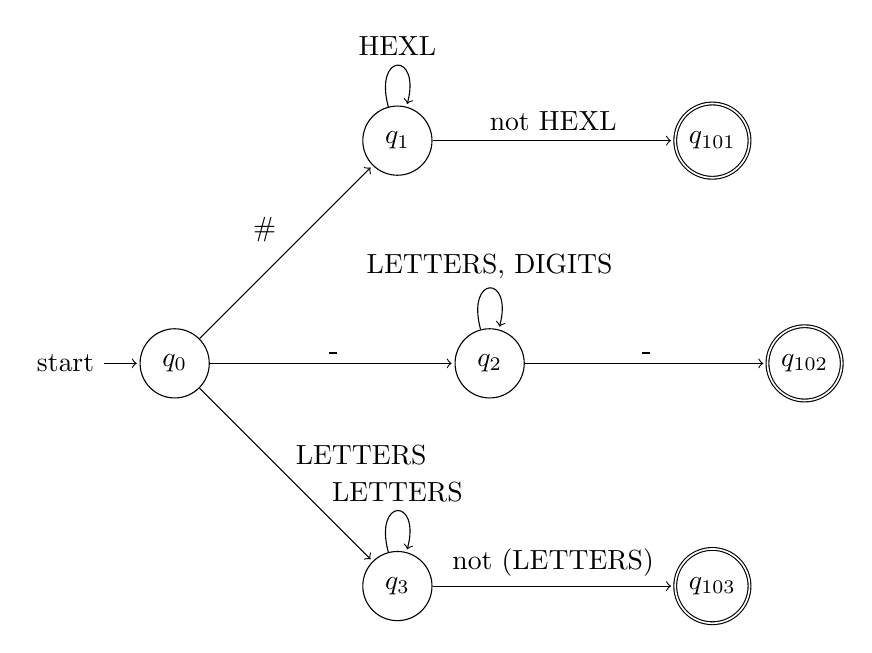
\begin{tikzpicture}[shorten >=1pt,node distance=4cm,on grid,auto] 
            \node[state, initial] (q_0) {$q_0$};
            \node[state] (q_1) [above right=of q_0] {$q_1$}; 
            \node[state] (q_2) [right=of q_0] {$q_2$}; 
            \node[state] (q_3) [below right=of q_0] {$q_3$}; 
            \node[state, accepting] (q_101) [right=of q_1] {$q_{101}$}; 
            \node[state, accepting] (q_102) [right=of q_2] {$q_{102}$}; 
            \node[state, accepting] (q_103) [right=of q_3] {$q_{103}$}; 
                \path[->] 
                (q_0) edge  node {\#} (q_1)
                    edge  node {\_} (q_2)
                    edge  node {LETTERS} (q_3)
                (q_1) edge  node  {not HEXL} (q_101)
                    edge [loop above] node {HEXL} ()
                (q_2) edge  node  {\_} (q_102)
                    edge [loop above] node {LETTERS, DIGITS} ()
                (q_3) edge [loop above] node {LETTERS} ()
                    edge  node  {not (LETTERS)} (q_103);
        \end{tikzpicture}
    \end{center}

    \section{Designing the transition matrix - Case II}
    Given the DFA defined for case II, propose a feasible transition matrix for such a DFA. 
    Remember to useindexes larger or equal to 100 to indicate goal states and the constant 
    \verb\ERROR\ for transitions leading to the error state.

    \begin{center}
        \begin{tabular}{c | c  c  c  c  c  c}
            & DIGITS & LETTERS & \# & '\_' & HEXL & other \\
            \hline
            
            $q_0$ & \verb\ERROR\ & $q_3$ & $q_1$ & $q_2$ & \verb\ERROR\ & \verb\ERROR\ \\
            $q_1$ & $q_{101}$ & $q_{101}$ & $q_{101}$ & $q_{101}$ & \verb\ERROR\ & \verb\ERROR\ \\
            $q_2$ & $q_2$ & $q_2$ & \verb\ERROR\ & $q_{102}$ & \verb\ERROR\ & $q_{101}$ \\
            $q_3$ & $q_{103}$ & $q_3$ & $q_{103}$ & $q_{103}$ & $q_{103}$ & \verb\ERROR\ \\
            
        \end{tabular}
    \end{center}
\end{document}